\documentclass[12pt]{article}
\usepackage{pdfpages}
\usepackage[T1]{fontenc}
\usepackage[utf8]{inputenc}
\usepackage{amsmath}
\usepackage{amsfonts}
\usepackage{amssymb}
\usepackage[top=1in, bottom=1in, left=1in, right=1in]{geometry}
\usepackage[numbered,framed]{matlab-prettifier}
\usepackage{graphicx}
\usepackage{textcomp}
\usepackage[export]{adjustbox}
\usepackage{bm}                          % Bold greek letters
\usepackage{float}                        % Forcing the figures to appear anywhere
\usepackage[hidelinks]{hyperref}  % TOC and internal links will be "hidden"
\usepackage[normalem]{ulem}      % For underlining
\usepackage{xcolor}                      % For the blue color

% Usage: \ghlink{URL}{Friendly Name}
\newcommand{\ghlink}[2]{\href{#1}{\color{blue}\uline{#2}}}

\lstset{
  style      = Matlab-editor,
  upquote    = true,
  showstringspaces=false
}

\title{WES 265 HW 1}
\author{Shantonu Mandal}
\date{\today}

\begin{document}

\begin{titlepage}
    \centering
    \vspace*{\fill}
    
    {\Huge \textbf{WES265 HW 1}} \\[0.5cm]
    {\Large Shantonu Mandal} \\[0.5cm]
    {\large \today}
    
    \vspace*{\fill} % Flexible space at the bottom (matches the top)
\end{titlepage}
\newpage


\tableofcontents
\newpage

\section*{1 \quad Problems from Intuitive Probability Book}
\addcontentsline{toc}{section}{1 \quad Problems from Intuitive Probability Book}

\subsection*{1. 4.19}
\addcontentsline{toc}{subsection}{1.1 4.19}
\label{subsec:1.1}
Let the events of interest be denoted as follows:
\begin{itemize}
    \item $R$: Rain occurs
    \item $S$: Sewer overflows
    \item $F$: Flooded road
\end{itemize}

\noindent \textbf{Given:} $P(S | R)=0.5$; $P(F|S)=0.3$; $P(R)=0.2$\\[10pt]
\noindent Notice that $F \subset S \subset R.$ That is, the road can only flood if the sewer overflows, and the sewer can only overflow if it rains.\\[10pt]
From set theory and subset properties, $S \cap R\ =\ S$ and $F \cap S\ =\ F$.\\[10pt]
\noindent Therefore,
\label{eq:prob_relations}
\begin{align}
    P(S|R) &= \frac{P(S)}{P(R)} \label{eq:sewer_rain} \\[10pt]
    P(F|S) &= \frac{P(F)}{P(S)} \label{eq:flood_sewer}
\end{align}
\begin{align*}
    P(F) &= P(F|S) \times P(S) \\[10pt]
    &= P(F|S) \times P(S|R) \times P(R) \quad \text{(from \eqref{eq:flood_sewer})} \\[10pt]
    &= 0.3 \times 0.5 \times 0.2 \\[10pt]
    \therefore P(F) &= 0.03
\end{align*}
The probability that road will flood is 3.0\%.

\subsection*{2. 4.28}
\addcontentsline{toc}{subsection}{1.2 4.28}
\label{subsec:1.2}

Only outcomes of the experiment are: success, failure, don't know \\[10pt]
$P(\text{success}) = 0.5$ and consequently, $P(\text{not success}) = 1 - 0.5 = 0.5$\\[10pt]
\noindent This is akin to a coin toss (2 events with equal probability of 0.5).
\begin{equation*}
    P(3 \text{ successes out of 5}): \binom{5}{3} \left(\frac{1}{2}\right)^5 = \frac{10}{32} = \frac{5}{16}
\end{equation*}
\noindent This can also be arrived at using the binomial probability law, as these trials are independent Bernoulli trials.

\subsection*{3. 4.29}
\addcontentsline{toc}{subsection}{1.3 4.29}
\label{subsec:1.3}

\lstinputlisting[style=Matlab-editor]{hw1_p1c.m}
\begin{figure}[H]
    \centering
    \makebox[\textwidth][c]{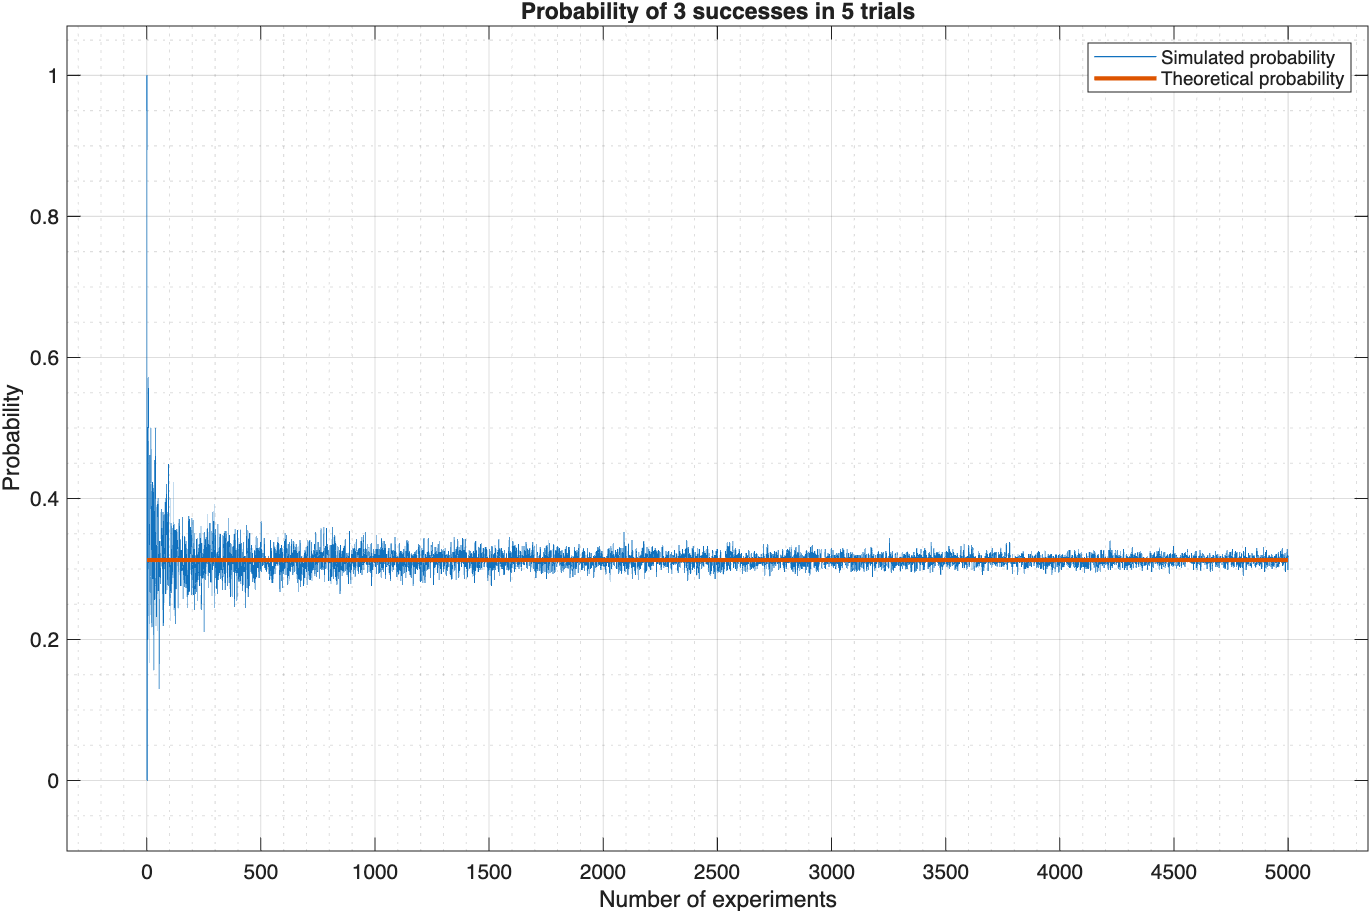
\includegraphics[width=1.2\textwidth]{Figure_p1c.png}}
    \caption{Graph for Problem 1.3}
    \label{fig:fig_p1c}
\end{figure}

\subsection*{4. 5.6}
\addcontentsline{toc}{subsection}{1.4 5.6}
\label{subsec:1.4}

$P_X[k] = \alpha p^k$ for $k=2,3,4,\dots$ \\[10pt]
For $P_X[k]$ to be a valid PMF, the following properties must hold:
\begin{align*}
    \sum_{k=-\infty}^{\infty} P_X[k] = 1\\[10pt]
    0 \le P_X[k] \le 1 \quad \forall \ k
\end{align*}

\noindent For the first property,
\begin{equation*}
    \sum_{k=2}^{\infty} \alpha \cdot p^k = 1 \implies \alpha(p^2 + p^3 + p^4 + \dots) = 1
\end{equation*}
Since $\alpha p^k > 0$ for every $k$, it follows that \bm{$\alpha > 0$}.\\
Also, since $\alpha p^k \le 1$, it follows that \bm{$0 < p < 1$}. Further, $\sum_{k} p^k$ is the sum of geometric progression with the ratio $p < 1$ and first term $p^2$:
\begin{align*}
    \alpha \sum_{k=2}^{\infty} p^k &= \alpha \cdot \frac{p^2}{1-p} = 1 \\
    \implies\alpha &= \frac{1-p}{p^2}
\end{align*}

\subsection*{5. 5.20}
\addcontentsline{toc}{subsection}{1.5 5.20}
\label{subsec:1.5}

$X \sim \text{Pois}(\lambda); Y = 2X$ \\
PMF of $X$:\\
\begin{align*}
    P_X[k] = exp(-\lambda) \frac{\lambda^k}{k!}, \quad k=0,1,2, \dots
\end{align*}

\noindent By definition, the RV Y can only take even values.
\begin{align*}
    P[X=k] &=  exp(-\lambda) \frac{\lambda^k}{k!}, \quad k=0,1,2,3, \dots \\
    \implies P[Y = 2X = y] &= P[X = y/2] =  exp(-\lambda) \frac{\lambda^{y/2}}{(y/2)!}
\end{align*}
\begin{equation*}
    \therefore P_Y[m] = \begin{cases} exp(-\lambda) \frac{\lambda^{m/2}}{(m/2)!}, & m=0,2,4, \dots \\[10pt] 0 & \text{otherwise} \end{cases}
\end{equation*}

\subsection*{6. 5.31}
\addcontentsline{toc}{subsection}{1.6 5.31}
\label{subsec:1.6}

Let X be the number of calls in a 1 minute interval. \\
$\lambda = \text{Arrival rate} \times T = 1 \times 60 = 60$
\begin{align*}
    P(X > 100) &= 1 - P(X \le 100) = 1 - \sum_{k=0}^{100} e^{-\lambda} \cdot \frac{\lambda^k}{k!} \\[10pt]
    &= 1 - e^{-\lambda}\left(1 + \frac{\lambda}{1!} + \frac{\lambda^2}{2!} + \dots + \frac{\lambda^{100}}{100!}\right)\\[10pt]
    &= 1 - F(100; 60), \quad where\ F\ =\ CDF\ of\ Poisson RV
\end{align*}

\lstinputlisting[style=Matlab-editor]{hw1_p1f.m}

\noindent \textbf{MATLAB Command Window Output:}
\begin{lstlisting}[
    basicstyle=\small\ttfamily, 
    frame=single, 
    backgroundcolor=\color{gray!10},
    breaklines=true,
    columns=fullflexible
]
P(More than 100 calls in a minute) = 8.685e-07
\end{lstlisting}


\subsection*{7. 11.10}
\addcontentsline{toc}{subsection}{1.7 11.10}
\label{subsec:1.7}

$X = A + U$, where $U \sim \mathcal{U}(-1/2, 1/2)$\\
\begin{align*}
    SNR &= \frac{E^2[X]}{Var(X)}\\[10pt]
    E[X] &= E[A + U] = E[A] + E[U] = A + 0 \\[10pt]
    Var(X) &= Var(A + U) = Var(U) \\[10pt]
    Var(X) &= \int_{-1/2}^{1/2} x^2 \cdot 1 \cdot dx = \left[\frac{x^3}{3}\right]_{-1/2}^{1/2} = \frac{1/8}{3} - \left(\frac{-1/8}{3}\right) = \frac{1}{12}
\end{align*}
\begin{equation*}
    \therefore SNR = 1000 = \frac{A^2}{1/12} \implies A = \sqrt{\frac{1000}{12}} = 10\sqrt{\frac{5}{6}} \approx 9.1287
\end{equation*}

\subsection*{8. 11.27}
\addcontentsline{toc}{subsection}{1.8 11.27}
\label{subsec:1.8}

\noindent \textbf{Given:} RV $X$ has the mixed PDF:
\[
p_X(x) = \frac{1}{2} \delta(x) + \frac{1}{\sqrt{2\pi\sigma^2}} exp\left(\frac{-x^2}{2\sigma^2}\right) u(x)
\]

\noindent
\begin{itemize}
    \item[] Discrete at $x=0$ with the Dirac delta function giving a probability of $0.5$ 
    \item[] Continuous for $x > 0$ with the random variable having a normal/Gaussian distribution 
\end{itemize}

\begin{align*}
    E[X^2] &= \int_{-\infty}^{\infty} x^2 p_X(x) dx \\[10pt]
    &= \int_{-\infty}^{\infty} x^2 \cdot \frac{1}{2} \delta(x) dx + \int_{0}^{\infty} x^2 \frac{1}{\sqrt{2\pi\sigma^2}} exp\left(\frac{-x^2}{2\sigma^2}\right) dx
\end{align*}
For the first term, using the sifting property of Dirac delta function:\\
\[
    \int_{-\infty}^{\infty} x^2 \delta(x) dx = 0
\]
Therefore,
\begin{align*}
    E[X^2] &= 0 + \int_{0}^{\infty} x^2 \frac{1}{\sqrt{2\pi\sigma^2}} exp\left(\frac{-x^2}{2\sigma^2}\right) dx\\[10pt]
    &= \frac{1}{\sqrt{2\pi\sigma^2}} \int_{0}^{\infty} x^2 exp\left(\frac{-x^2}{2\sigma^2}\right) dx\\[10pt]
\end{align*}
Using $uv$ rule or integration by parts:
\[
\int u \cdot dv = uv - \int v \cdot du
\]
With the LIATE rule, let u and v be the following:
\begin{itemize}
    \item[]
    \[
    u=x, \quad dv=x \cdot exp\left(\frac{-x^2}{2\sigma^2}\right) dx, \quad du = dx
    \]
    \item[]
    \[
    v = \int x \cdot exp\left(\frac{-x^2}{2\sigma^2}\right) dx
    \]
\end{itemize}

\noindent To solve this integral for $v$, notice that 
\begin{align*}
    \frac{d}{dx} \left( \exp\left\{-\frac{x^2}{2\sigma^2}\right\} \right) &= \exp\left(-\frac{x^2}{2\sigma^2}\right) \cdot \left( -\frac{2x}{2\sigma^2} \right) \\[10pt]
    &= -\frac{1}{\sigma^2} \cdot x \cdot \exp\left(-\frac{x^2}{2\sigma^2}\right) \\[15pt]
    \therefore v = \int x \cdot \exp\left(-\frac{x^2}{2\sigma^2}\right) \, dx &= -\sigma^2 \cdot \exp\left(-\frac{x^2}{2\sigma^2}\right)\\[10pt]
\end{align*}

\noindent Substituting this back into $E[X^2]$:
\begin{align*}
    E[X^2] &= \frac{1}{\sqrt{2\pi\sigma^2}} \left( \left[-x \sigma^2 exp\left(\frac{-x^2}{2\sigma^2}\right)\right]_0^\infty + \sigma^2 \int_0^\infty exp\left(\frac{-x^2}{2\sigma^2}\right) dx \right) \\[10pt]
    &= \frac{1}{\sqrt{2\pi\sigma^2}} \left( 0 + \sigma^2 \int_0^\infty exp\left(\frac{-x^2}{2\sigma^2}\right) dx \right) \\[10pt]
    &= \frac{\sigma}{\sqrt{2\pi}} \int_0^\infty exp\left(\frac{-x^2}{2\sigma^2}\right) dx
\end{align*}

\noindent To evaluate this integral:
\begin{align*}
    z = \frac{x}{\sqrt{2}\sigma} &; \quad dz = \frac{dx}{\sqrt{2}\sigma} ; \quad z^2 = \frac{x^2}{2\sigma^2} & \\[10pt]
    \implies E[X^2] &= \frac{\sigma}{\sqrt{2\pi}} \int_{0}^{\infty} exp(-z^2) \cdot \sqrt{2}\sigma \, dz \\[10pt]
    &= \frac{\sigma^2}{\sqrt{\pi}} \int_{0}^{\infty} exp(-z^2) \, dz \\
\end{align*}

\noindent Now, let I be $\int_{-\infty}^{\infty} exp(-x^2) \, dx$ \\
\begin{align*}
    I^2 &= \int_{-\infty}^{\infty} exp(-x^2) \, dx \cdot \int_{-\infty}^{\infty} exp(-y^2) \, dy \\[10pt]
    &= \int_{-\infty}^{\infty} \int_{-\infty}^{\infty} exp(-(x^2 + y^2)) \, dx \, dy\\
\end{align*}
\noindent Converting to polar coordinates:
\begin{align*}
    x &= r \cos\theta\\
    y &= r \sin\theta \\
    x^2 + y^2 &= r^2\\
    dx \cdot dy &= r dr \cdot d\theta
\end{align*}
\noindent $\theta : 0 \to 2\pi \quad \& \quad r : 0 \to \infty$ \\
\[
I^2 = \int_{0}^{2\pi} \int_{0}^{\infty} exp(-r^2) r \, dr \, d\theta
\]

\begin{align*}
    I^2 &= \int_{0}^{2\pi} \left( \int_{0}^{\infty} r \cdot exp(-r^2) \, dr \right) \, d\theta \\[10pt]
    &= \int_{0}^{2\pi} \left[ -\frac{exp(-r^2)}{2} \right]_{0}^{\infty} \, d\theta \\[10pt]
    &= \int_{0}^{2\pi} \frac{1}{2} \, d\theta = \frac{1}{2} \left[ \theta \right]_{0}^{2\pi} \\[10pt]
    I^2 &= \pi \\[5pt]
    \therefore I &= \int_{-\infty}^{\infty} e^{-x^2} \, dx = \sqrt{\pi}
\end{align*}

\noindent Since $exp(-x^2)$ is even/symmetric,\\
\[
\int_{0}^{\infty} exp(-x^2) \, dx = \frac{\sqrt{\pi}}{2}
\]

\noindent Substituting this back into $E[X^2]$:
\begin{align*}
    E[X^2] &= \frac{\sigma^2}{\sqrt{\pi}} \int_{0}^{\infty} exp(-z^2) \, dz \\[10pt]
    &= \frac{\sigma^2}{\sqrt{\pi}} \cdot \frac{\sqrt{\pi}}{2} \\[10pt]
    \therefore E[X^2] &= \frac{\sigma^2}{2}\\
 \end{align*}
 
\noindent The result makes sense because the mixed PDF is essentially the positive half ($x \ge 0$) of a normal distribution with mean 0 and variance $\sigma^2$.
\\[10pt]
\noindent The PDF can be physically interpreted as the average power of a half-wave rectifier with input being a noise signal with PDF $\mathcal{N}(0, \sigma^2)$.

\subsection*{9. 11.46}
\addcontentsline{toc}{subsection}{1.9 11.46}
\label{subsec:1.9}

\lstinputlisting[style=Matlab-editor]{hw1_p1i.m}
\begin{figure}[H]
    \centering
    \makebox[\textwidth][c]{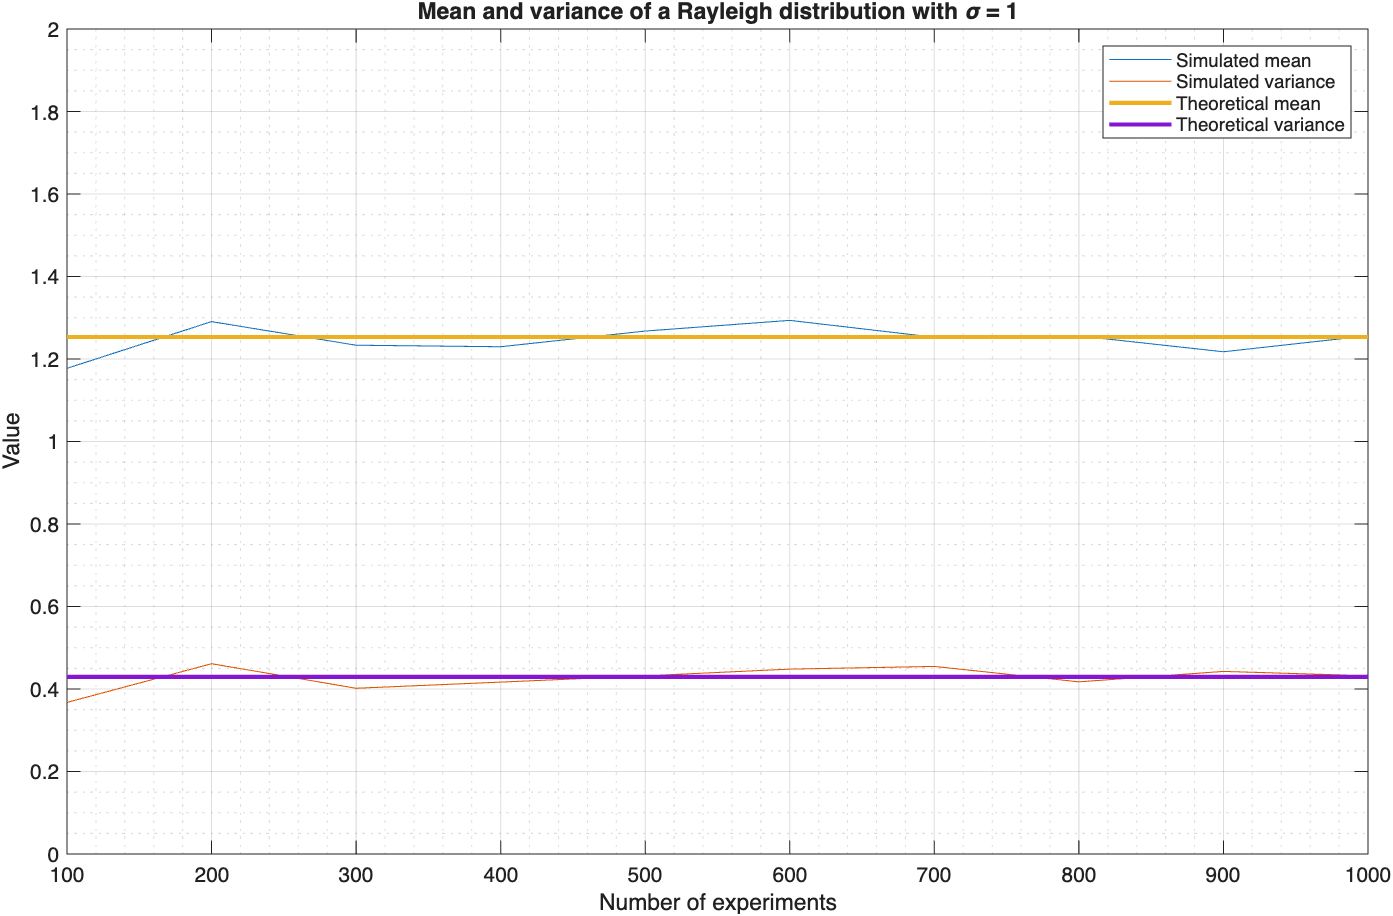
\includegraphics[width=1.2\textwidth]{Figure_p1i.png}}
    \caption{Graph for Problem 1.9}
    \label{fig:fig_p1i}
\end{figure}

\section*{2 \quad Linear Transformations of Random Variables}
\addcontentsline{toc}{section}{2 \quad Linear Transformations of Random Variables}

$Z = aX + b$

\subsection*{1. Mean}
\addcontentsline{toc}{subsection}{2.1 Mean}
\label{subsec:2.1}

\begin{align*}
    E[Z] &= E[aX + b]\\[10pt]
    &= a E[x] + b\\[10pt]
    &= a\mu + b
\end{align*}

\subsection*{2. Variance}
\addcontentsline{toc}{subsection}{2.2 Variance}
\label{subsec:2.2}

\begin{align*}
    Var(Z) &= Var(aX + b)\\[10pt]
    &= a^2 Var(x)\\[10pt]
    &= a^2\sigma^2\\
\end{align*}

\subsection*{3. Variance by definition}
\addcontentsline{toc}{subsection}{2.3 Variance by definition}
\label{subsec:2.3}

\begin{align*}
    Var(Z) &= E[Z^2] - (E[Z])^2\\[10pt]
    &= E[(aX+b)^2] - (a\mu + b)^2\\[10pt]
    &= E[(a^{2}X^2+b^2 + 2aXb)] - (a\mu + b)^2\\[10pt]
    &= a^2 E[X^2] + b^2 + 2aE[X]b - (a\mu + b)^2 \\[10pt]
    &= a^2 E[X^2] + b^2 + 2a\mu b - a^2\mu^2 - b^2 - 2a\mu b \\[10pt]
    &= a^2(E[X^2] - \mu^2) = a^2\sigma^2
\end{align*}

\newpage
\section*{3 \quad Expectation and Variance from a PDF}
\addcontentsline{toc}{section}{3 \quad Expectation and Variance from a PDF}
\label{sec:prob3}

$p_X(x) = \begin{cases} 2x & x \in [0,1] \\ 0 & \text{otherwise} \end{cases}$

\subsection*{1. Verify that $p_X(x)$ is a valid probability density function.}
\addcontentsline{toc}{subsection}{3.1 PDF validity check}
\label{subsec:3.1}

a) PDF must be non-negative: $p_x(x) \ge 0$. This condition is clearly satisfied. \\[10pt]
b) PDF must integrate to 1:
\begin{itemize}
    \item[] \[\int_{-\infty}^{\infty} p_X(x) dx = 1\]
    \item[] \[\int_0^1 (2x) dx = \left[x^2\right]_0^1 = 1\]
\end{itemize}

\subsection*{2. Mean}
\addcontentsline{toc}{subsection}{3.2 Mean}
\label{subsec:3.2}

\begin{align*}
    E[X] &= \int_{-\infty}^{\infty} x\cdot p_X(x)dx\\[10pt]
    &= \int_0^1 x \cdot 2x dx\\[10pt]
    &= 2 \int_0^1 x^2 dx\\[10pt]
    \therefore E[X] &= 2\left[\frac{x^3}{3}\right]_0^1 = \frac{2}{3}
\end{align*}

\subsection*{3. Variance}
\addcontentsline{toc}{subsection}{3.3 Variance}
\label{subsec:3.3}

\text{Variance, $Var(X) = E[X^2] - (E[X])^2$}
\begin{align*}
    E[X^2] &= \int_0^1 x^2 \cdot 2x dx = 2 \int_0^1 x^3 dx = 2\left[\frac{x^4}{4}\right]_0^1 = \frac{1}{2} \\
    \therefore Var(X) &= \frac{1}{2} - \left(\frac{2}{3}\right)^2 = \frac{1}{2} - \frac{4}{9} = \frac{1}{18}\\
\end{align*}

\section*{4 \quad Empirical vs Theoretical Determination of Probability}
\addcontentsline{toc}{section}{4 \quad Empirical vs Theoretical Determination of Probability}
\label{sec:prob4}

\lstinputlisting[style=Matlab-editor]{hw1_p4.m}

\noindent \textbf{MATLAB Command Window Output:}
\begin{lstlisting}[
    basicstyle=\small\ttfamily, 
    frame=single, 
    backgroundcolor=\color{gray!10},
    breaklines=true,
    columns=fullflexible
]
Empirical P[-1 <= X <= 1] = 0.68272
Theoretical P[-1 <= X <= 1] = 0.68269 
\end{lstlisting}

\begin{figure}[H]
    \centering
    \makebox[\textwidth][c]{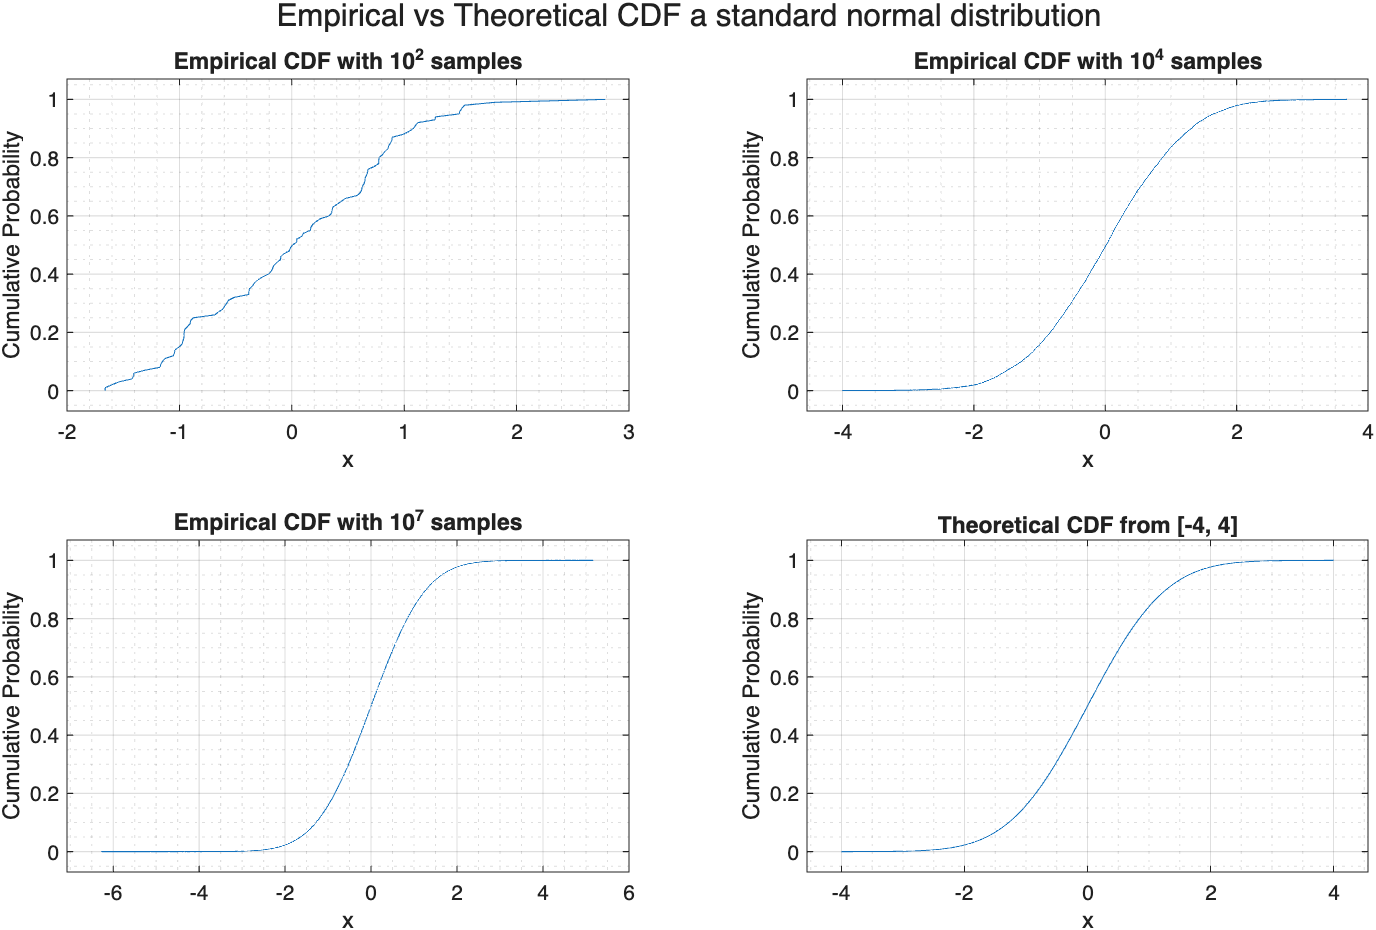
\includegraphics[width=1.2\textwidth]{Figure_p4.png}}
    \caption{Graphs for Problem 4}
    \label{fig:fig_p4}
\end{figure}

\section*{5 \quad Notes}
\addcontentsline{toc}{section}{5 \quad Notes}
\label{sec:notes}

All of my MATLAB\textsuperscript{\textregistered} and \LaTeX \ source code is uploaded to \ghlink{https://github.com/ShantonuM/wes265_sp2026/tree/main/hw1}{GitHub}.\\[10pt]
For better readability, I converted my handwritten notes to  \LaTeX \ using generative AI. Although, I had to heavily modify the output and check thoroughly for accuracy.\\[10pt]
Below are my handwritten notes for reference.

\newgeometry{margin=0in} % Kills all margins immediately


\includepdf[pages=-, fitpaper=true]{hw1_handwritten_1.pdf}

\includepdf[pages=-, fitpaper=true]{hw1_handwritten_2.pdf}

\end{document}